% \documentclass[9pt,compress,handout]{beamer}
\documentclass[9pt,compress]{beamer}
\usepackage{xcolor}
\usepackage{listings}
\usepackage[lined,frenchkw]{algorithm2e}
\usepackage{ifthen}  %%% for comments
\usepackage{amssymb}  %%% for comments
\usepackage{soul}  %%% for strikethrough

\lstset{showstringspaces=false}
 
% comments \nb{label}{color}{text}
\newboolean{showcomments}
\setboolean{showcomments}{true}
\ifthenelse{\boolean{showcomments}}
	{\newcommand{\nb}[3]{
		{\colorbox{#2}{\bfseries\sffamily\scriptsize\textcolor{white}{#1}}}
		{\textcolor{#2}{\sf\small$\blacktriangleright$\textit{#3}$\blacktriangleleft$}}}
	 \newcommand{\version}{\emph{\scriptsize$-$Id$-$}}}
	{\newcommand{\nb}[3]{}
	 \newcommand{\version}{}}
\newcommand{\sd}[1]{\nb{Stephane}{red}{#1}}
\newcommand{\sv}[1]{\nb{Steven}{blue}{#1}}
\newcommand{\oz}[1]{\nb{Oleks}{olive}{#1}}


\beamertemplatenumberedballsectiontoc

\addtobeamertemplate{navigation symbols}{}{%
    \usebeamerfont{footline}%
    \usebeamercolor[fg]{footline}%
    \setbeamercolor{footline}{fg=black}
	\setbeamerfont{footline}{series=\bfseries}
    \hspace{1em}%
    \insertframenumber/\inserttotalframenumber
    
   
}
\AtBeginSection[]
{
  \begin{frame}<beamer>
    \frametitle{Plan}
    \small\tableofcontents[currentsection,subsectionstyle=hide/hide/hide]
  \end{frame}
}

\AtBeginSubsection[] % Do nothing for \subsection* 
{ 
\begin{frame}<beamer> 
\frametitle{Plan}
\small\tableofcontents[currentsection,currentsubsection,subsectionstyle=show/shaded/hide] 
\end{frame} 
}

\newcommand{\lectureTitle}{A practical introduction with Pharo and PharoThings}
\title{IOT\\
  {\small --- \lectureTitle\ ---}\vskip-0.5em}

\author{
\small Steven Costiou\\
  \footnotesize steven.costiou@inria.fr\\
  ~~\\
  \small Allex Oliveira\\
  \footnotesize allex.oliveira@inria.fr\\
  ~~\\
}

\date{\today}

\begin{document}
\frame[plain]{\titlepage}

\frame{\frametitle{Plan}
 % \setcounter{tocdepth}{2}
 \tableofcontents
}

\section{About this course} 

\frame{\frametitle{About this course}

This is a practical introduction to IOT: we will learn how to write high-level software for sensors and how to use them in applications deployed on Raspberry-pi computers.\\
~~\\
\pause
\begin{block}
{We will learn to:}

		\begin{itemize}
			\item Program with Pharo and PharoThings on Raspberry-pi computers,
			\item design and implement software models of sensors,% and motors,
			\item write applications using sensors,% and motors,
			\item use Pharo remote development tools to debug running IOT applications.
			
		\end{itemize}
		\end{block}
\pause
\begin{block}{Want more?}
\begin{itemize}
			\item A MOOC with more theoretical aspects: \url{https://www.coursera.org/learn/iot/}
			\item PharoThings materials: \url{https://github.com/SquareBracketAssociates/Booklet-APharoThingsTutorial}
\end{itemize}
\end{block}
}

\section{IOT: some generalities} %

\frame{\frametitle{What is IOT?}

\begin{block}{Internet of Things}

		\begin{itemize}
			\item Objects inter-connected through the internet:\\
			~\\
				\begin{itemize}	
			\item Objects are unique entities sharing data in a network:\\ a person, a phone, a device...\\
			~\\
			\item Device:\\ hardware (micro-computer, sensors, motors...) + software (\textit{intelligence}),\\
			~\\
			\item Objects are interrelated:\\ they transfer data between them through the network\\			
			~\\
			\item Objects use a protocol to communicate:\\ for example, an HTTP REST API through TCP/IP...\\
			~\\
			\item Objects need a power source to be autonomous\\
			
		\end{itemize}
			
		\end{itemize}
		\end{block}

}

\frame{\frametitle{What is IOT?}

\begin{block}{Examples of IOT systems/applications}

		\begin{itemize}
			\item Personal health or sport monitoring systems\\
			~\\
			\item Smart homes: your fridge now tells you when you need to refill!\\
			~\\
			\item Logistics: automated warehouses and production chain monitoring\\
			~\\
			\item Smart grids: optimizing energy production and routing\\
			~\\
			\item Etc.\\		
		\end{itemize}
		\end{block}
}

\section{Sensors and actuators} %

\frame{\frametitle{Sensors}


	
	\textit{"A sensor is a device, module, machine, or subsystem whose purpose is to detect events or changes in its environment and send the information to other electronics, frequently a computer processor."}
	\begin{flushright}
	$-$ https://en.wikipedia.org/wiki/Sensor
	\end{flushright}
	\begin{block}{ }
		\begin{itemize}
			\item Transforms a physical information (\textit{e.g.}, the temperature of the room) to an analog or digital signal
			\item The analog/digital signals are processed by the computer processor and interpreted and used by user-applications
			\item Sensors are sources of data (inputs) in IOT applications

		\end{itemize}
		\end{block}
		\pause
		\begin{block}{Examples}
		\begin{itemize}
			\item Temperature sensor: measures temperature in an environment
			\item Camera
			\item Accelerometer: measures acceleration
			\item ...

		\end{itemize}
		\end{block}
}

\frame{\frametitle{Sensors}
	
	\begin{block}{What do sensors measure?}
		\begin{itemize}
			\item One sensor only measure one specific property of its environment
			\item Ideally, a sensor should not interfere with the environment (\textit{i.e.}, not influence the measured value)
			\item Sensors always work in association with an electronic system (in IOT)

		\end{itemize}
	\end{block}
		\pause
		\begin{block}{How do sensors measure?}
	\begin{center}
	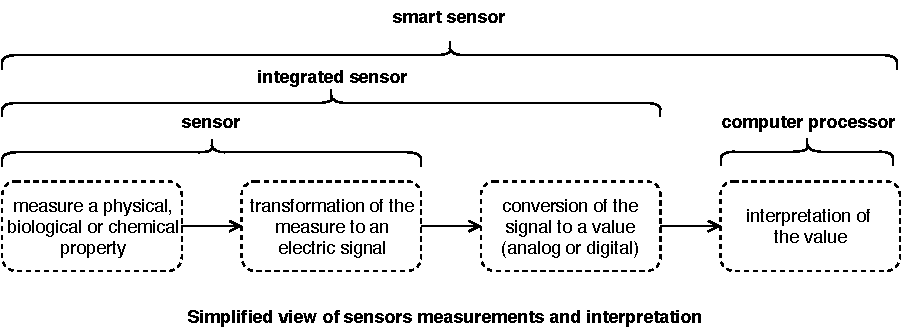
\includegraphics[width=1\linewidth]{../images/sensors}
	\end{center}
		\end{block}
}

\frame{\frametitle{Sensors}	
	
		
		\begin{block}{Different kind of sensors}
		\begin{itemize}
			\item \textbf{Basic sensor element: transforms a physical phenomenon into an electronic signal}\\
			Example: RTD\footnote{Resistance Temperature Detector}s measure the resistance of metal, that changes with temperature\\
			~\\
			\item \textbf{Integrated sensor: sensor element with signal conditioning}\\
			Example:  A sensor that transforms the resistance measured by a RTD into an analog signal (e.g., 0 to 1023)\\
			~\\
			\item \textbf{Smart or intelligent sensor: integrated sensor with additional features}\\
			Example:  A sensor that transforms the analog value transformed from an RTD resistance into a human-readable temperature in Celsius

		\end{itemize}
		\end{block}
		

}

\frame{\frametitle{Actuators}

\begin{block}{Systems that physically interact with the environment}

		\begin{itemize}
			\item Controlled by an electrical signal\\
			~\\
			\begin{itemize}
			\item Transforms the signal into a mechanical motion (output)\\
			~\\
			\item Requires a power source\\
			~\\
			
		\end{itemize}
		\item Has a direct impact on the environment\\
			~\\
		\begin{itemize}
			\item An actuator can affect sensors!			
		\end{itemize}
				
		\end{itemize}
		\end{block}
		
				\begin{block}{Examples}
		\begin{itemize}
			\item LED: produces light
			\item Motor: induces movement
			\item Speaker: produces sound
			\item ...

		\end{itemize}
		\end{block}
}



\section{The Raspberry-pi computer} %
\frame{\frametitle{The Raspberry-pi single-board computer}

\begin{block}{Cheap general-purpose single-board computer}

		\begin{itemize}
			\item ARM processor
			\item Linux based distributions or Windows IOT operating systems
			\item 40 GPIO (general-purpose input/output) pins to control sensors/actuators
		
		\end{itemize}
		\end{block}
		
			\begin{center}
		
			\begin{figure}
			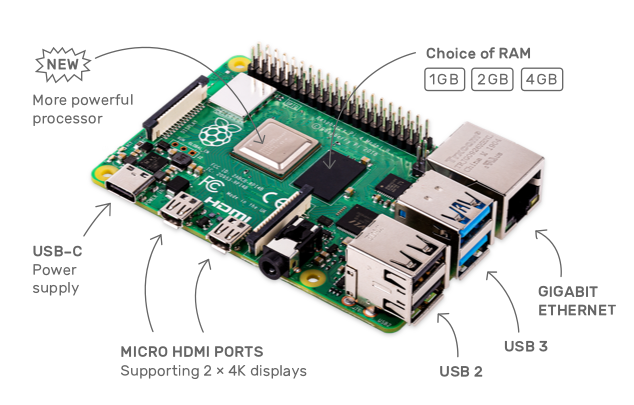
\includegraphics[scale=0.25]{../images/pi4}			
			\caption{https://www.raspberrypi.org/products/raspberry-pi-4-model-b/}	
			\end{figure}
	
	\end{center}
}

\frame{\frametitle{Raspberry-pi's GPIO}


\begin{block}{General properties of GPIO pins}

		\begin{itemize}
			\item Pins can be configured as \texttt{input} (e.g., to read sensors) or as \texttt{output}
			\item Values set to outputs or read as input can be set to \texttt{high}, or \texttt{1} (3.3V) or \texttt{low}, or \texttt{0} (0V)
			\item 4 hardware PWM (Pulse-Width Modulation) pins: control of the voltage by switching power on and off  at a fast rate\footnote{\url{https://en.wikipedia.org/wiki/Pulse-width_modulation}} 
			\item SPI (Serial Peripheral Interface): synchronous serial communication interface between a master and a slave\footnote{\url{https://en.wikipedia.org/wiki/Serial_Peripheral_Interface}}
			\item I2C (Inter-Integrated Circuit): synchronous, multi-master, multi-slave, packet switched, single-ended, serial computer bus\footnote{\url{https://en.wikipedia.org/wiki/I\%C2\%B2C}}
			\item 2 serial pins (transmission and reception)
		\end{itemize}
		\end{block}
}
\frame{\frametitle{Example projects based on Raspberry-pi and Pharo-Things}

\includegraphics[width=\linewidth]{../images/projects}
}

\section{IOT with PharoThings} %

\frame{\frametitle{PharoThings}

	\begin{center}
	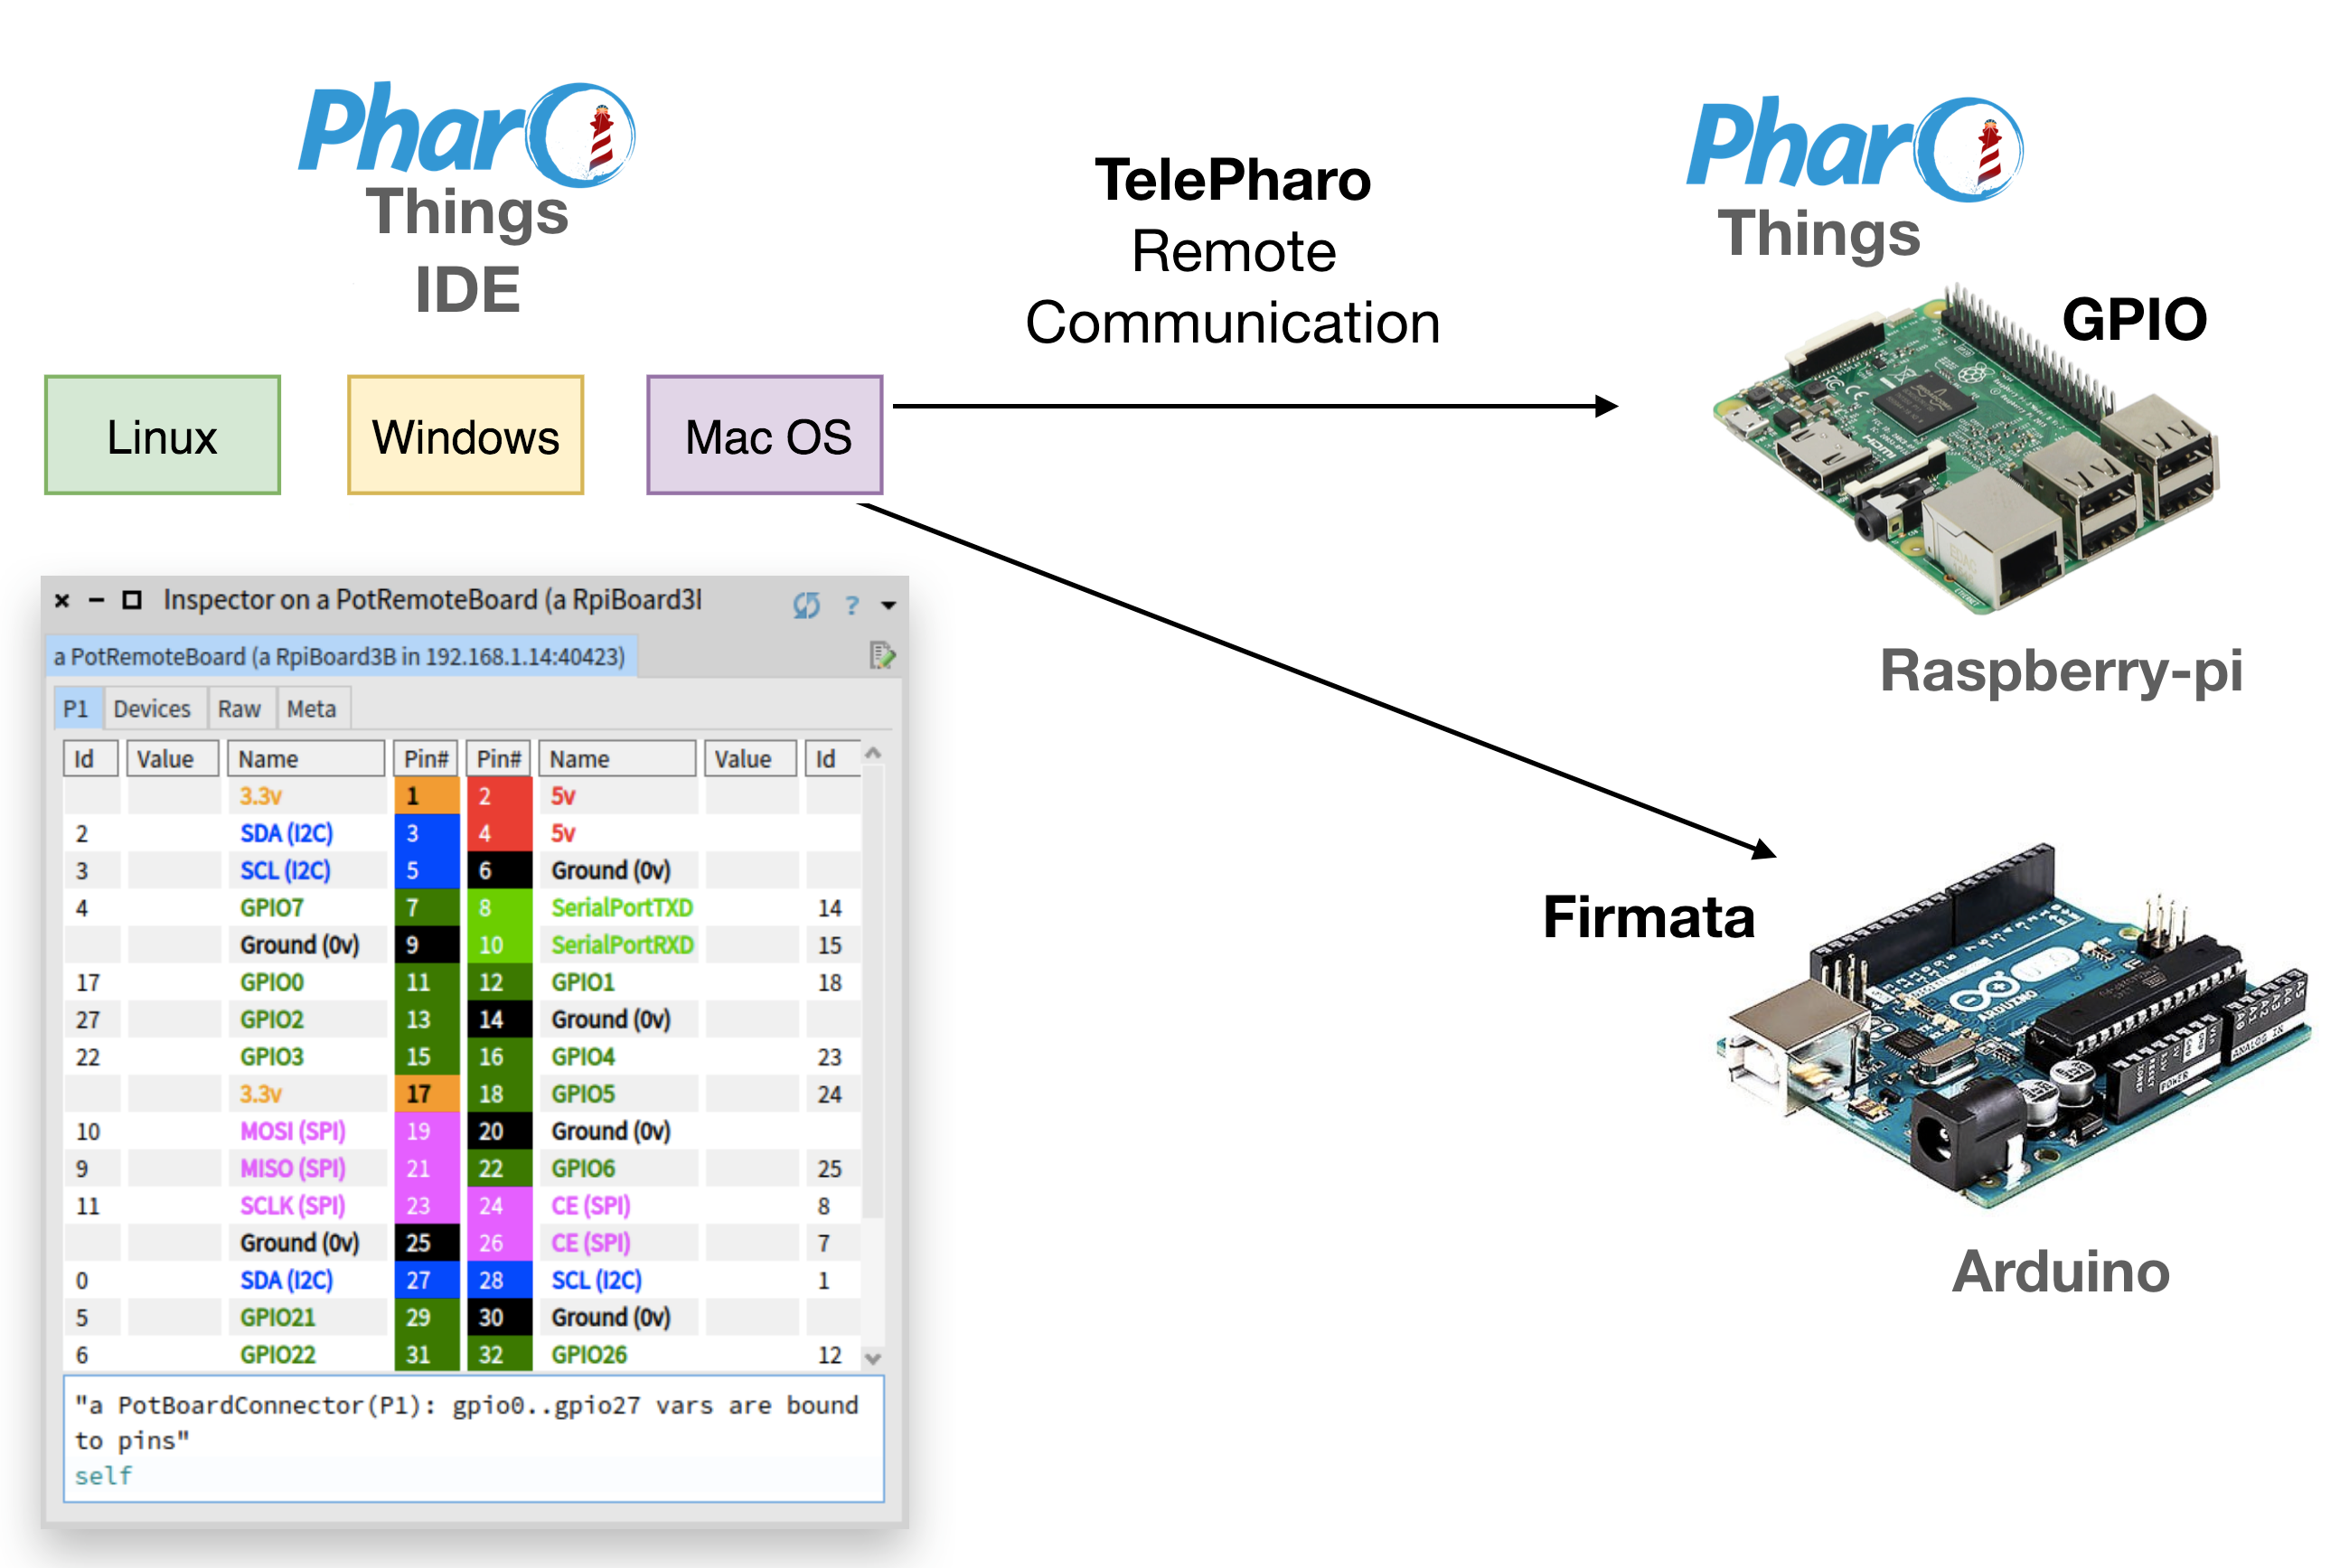
\includegraphics[width=1\linewidth]{../images/pthings-illustration}
	\end{center}
}

\frame{\frametitle{The PharoThings infrastructure}
\begin{block}{Developers (clients) connect to running IOT devices (servers)}
	\begin{itemize}
		\item Developers connect to remote IOT devices running their application 
		\item Pharo development and debugging tools are remotely usable through the TelePharo architecture
		\item Developers can connect to many devices at the same time from their development machine
			
	\end{itemize}
	\end{block}

	\begin{center}
	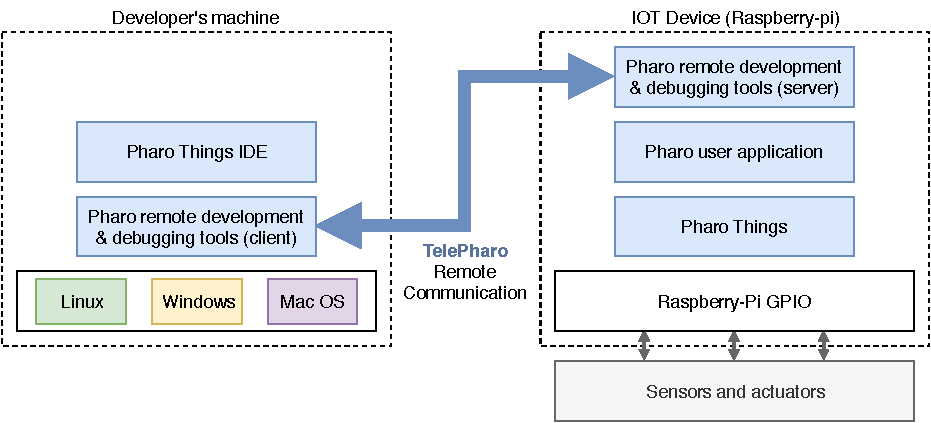
\includegraphics[width=1\linewidth]{../images/pharo-things-arch}
	\end{center}
}

\frame{\frametitle{PharoThings development process}

\begin{enumerate}
			\item Developers connect to running IOT application, deployed on IOT devices (Raspberry-pi)
			\item Developers remotely and lively write, test and debug code
			\item When development or debugging is finished, developers disconnect from the device
			\item At any point developers can reconnect and start or continue developing their IOT app $-$ which is still running!\\
			~\\
		\end{enumerate}
	\begin{center}
	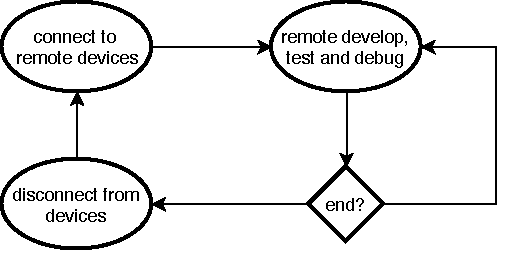
\includegraphics[scale=0.75]{../images/pharo-things-dev-process}
	\end{center}	

}

\frame{\frametitle{PharoThings tools}

\begin{block}{Remote development and debugging tools}
	\begin{itemize}
		\item Playground: write scripts and execute code
		\item Class browser: write classes and applications
		\item Inspector:
			\begin{itemize}
			\item observe your application state
			\item observe and interact with remote live objects
			\item observe and control GPIO state			
			\end{itemize}
		\item Debugger: debug and fix your code (live!)
		\item Process browser: inspect and control running processes			
	\end{itemize}
	\end{block}


}
\section{PharoThings in practice}

\frame[containsverbatim]{\frametitle{Downloading and starting PharoThings on the Raspberry-pi}

\begin{block}{On a running Raspbian on your Raspberry Pi}

Open a terminal window in your Raspberry Pi (local or through remote SSH) and enter the following commands:

\begin{lstlisting}
wget -O - get.pharoiot.org/server | bash
\end{lstlisting}	

This downloads the server side and extracts the files to the \texttt{pharoiot-server} folder.
The following commands will go to that folder and run the server:

\begin{lstlisting}
cd pharoiot-server
./pharo-server
\end{lstlisting}	

\begin{itemize}
			\item You should see this message: \texttt{a TlpRemoteUIManager is registered on port 40423}.
			\item This means that you have the TelePharo architecture running on your Raspberry on TCP port 40423 !
			\item Now you can use Pharo IoT on your computer to connect to your Raspberry and create IoT applications remotely.			
			\end{itemize}
\end{block}
}

\frame[containsverbatim]{\frametitle{Connecting to a remote device}

\begin{block}{On a running Raspbian on your Raspberry Pi}

\begin{itemize}
			\item First download the PharoThings IDE on your Windows/Linux/Mac computer \url{get.pharoiot.org/multi.zip} and run Pharo
			\item Open a playground in your local pharo image
			\item Write and \texttt{doIt} the following:			
\end{itemize}
			
\begin{lstlisting}
remotePharo := TlpRemoteIDE connectTo: 
	(TCPAddress ip: #[192 168 1  200] port: 40423).
\end{lstlisting}	

If you don’t receive any error, this means that you are connected. The \texttt{remotePharo} object allows you to interact with the remote device.

%\begin{lstlisting}
%remotePharo openPlayground.
%remotePharo openBrowser.
%remotePharo openProcessBrowser.
%\end{lstlisting}	


\end{block}
}

\frame[containsverbatim]{\frametitle{Inspecting the physical board (1)}

\begin{block}{We can inspect the software model of the remote device}

\begin{itemize}
			\item We must select the model corresponding to physical board
			\begin{itemize}
				\item \texttt{RpiBoardBRev1}: Raspberry Pi Model B Revision 1
				\item \texttt{RpiBoardBRev2}: Raspberry Pi Model B Revision 2
				\item \texttt{RpiBoard3B}: Raspberry Pi Model B+, Pi2 Model B, Pi3 Model B, Pi3 Model B+		
\end{itemize}
			\item In the playground on your local image, evaluate the following:		
\end{itemize}

\begin{lstlisting}
remoteBoard := remotePharo evaluate: [ RpiBoard3B current].
\end{lstlisting}	

\begin{itemize}
				\item \texttt{RpiBoard3B} is a class from the remote system 
				\item \texttt{RpiBoard3B current} returns the current instance of the board
				\item \texttt{evaluate:}  remotely evaluates the block of code and returns the result
				\item \texttt{remoteBoard} stores that result, a remote instance of \texttt{RpiBoard3B}			
				
\end{itemize}

\end{block}

}

\frame[containsverbatim]{\frametitle{Inspecting the physical board (2)}

\begin{block}{We can inspect the software model of the remote device}
\begin{itemize}
				\item Evaluate \texttt{remoteBoard inspect} to observe the state of the board 
				\item The board inspector shows a layout of pins similar to Raspberry Pi docs
				\item This is a live tool which represents the current pins state			
\end{itemize}
	\begin{center}
	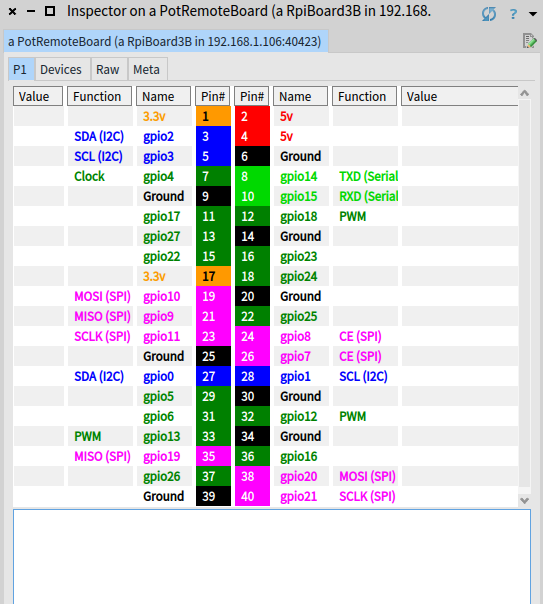
\includegraphics[width=0.5\linewidth]{../images/PharoThingsInspector}
	\end{center}	

\end{block}

}

\frame[containsverbatim]{\frametitle{Using GPIO: set a pin state (1)}

\begin{itemize}
				\item Digital pins can be set to \texttt{HIGH} (1) or \texttt{LOW} (0)
				\item They are shown with green/red icons which represent \texttt{HIGH}/\texttt{LOW}
				\item Digital pins' values are set using the \texttt{value:} message send to a pin
				\item Execute the following code in the lower pane of the board inspector:	icons are updated according to pin value changes
\end{itemize}


\begin{lstlisting}
	pin := gpio4.
	pin beDigitalOutput.
	pin value: 1
\end{lstlisting}	
}

\frame{\frametitle{Using GPIO: set a pin state (2)}

\begin{itemize}
				\item Results are visible in the board inspector:			
\end{itemize}
	\begin{center}
	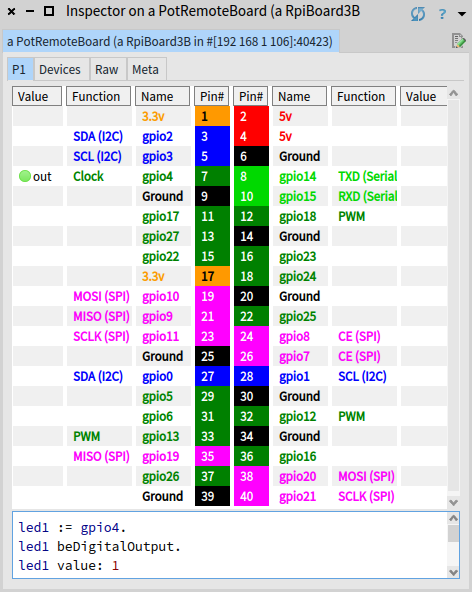
\includegraphics[width=0.5\linewidth]{../images/PharoThingsInspector-output}
	\end{center}
}


\frame[containsverbatim]{\frametitle{Using GPIO: read a pin state (1)}

\begin{itemize}
				\item Digital pins can be configured as inputs, possible states: \texttt{HIGH} (1)/\texttt{LOW} (0)
				\item Digital pins' values are read using the \texttt{value} message send to a pin
				\item Output pins also respond to \texttt{value}, and return the last set state
				\item Write the following code in the lower pane of the board inspector, and execute it:
\end{itemize}

\begin{lstlisting}
	inputPin := gpio17.
	inputPin beDigitalInput.
	inputPin value inspect
\end{lstlisting}	

}

\frame{\frametitle{Using GPIO: read a pin state (2)}

\begin{itemize}
				\item Results are visible in the board inspector:			
\end{itemize}
	\begin{center}
	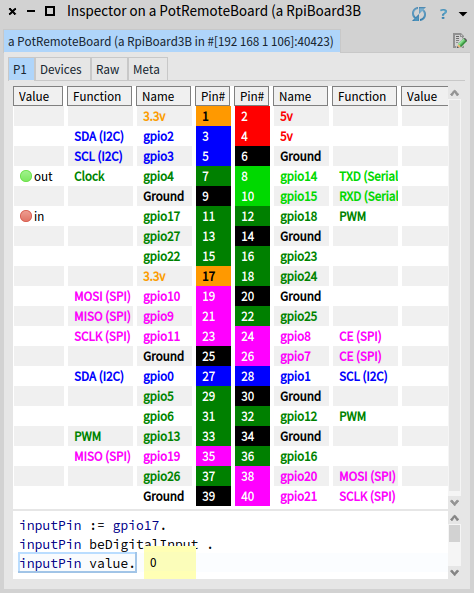
\includegraphics[width=0.5\linewidth]{../images/PharoThingsInspector-input}
	\end{center}
}


\frame[containsverbatim]{\frametitle{Scripting with the remote playground}

%show the gpio stuff with the playground
\begin{block}{Writing and reading GPIO from the remote playground}
\begin{itemize}
				\item We can interact with the GPIO in scripts and programs 
				\item Open locally a remote playground: \texttt{remotePharo openPlayground}
				\item The remote playground opens, now get the current board instance:
\end{itemize}

\begin{lstlisting}
	board := RpiBoard3B current.	
\end{lstlisting}	

\begin{itemize}
				\item Configure a new digital pin with the current board instance	:			
\end{itemize}

\begin{lstlisting}
	pin := board pinWithId: 7.
\end{lstlisting}	

\begin{itemize}
				\item Set the pin as output, set a \texttt{HIGH} value, inspect the state of the pin:
\end{itemize}

\begin{lstlisting}
	pin beDigitalOutput.
	pin value: 1.
	pin value inspect
\end{lstlisting}	

\end{block}
}


\frame{\frametitle{Developing with the remote class browser}
\begin{block}{Develop your applications with the remote class browser}
\begin{itemize}
				\item Write a package 
				\item Write a class with a method that increases a counter
				\item Use the remote playground to instantiate your class and play with your counter
				\item Save your remote code modifications: \texttt{remotePharo saveImage}
\end{itemize}

	\begin{center}
	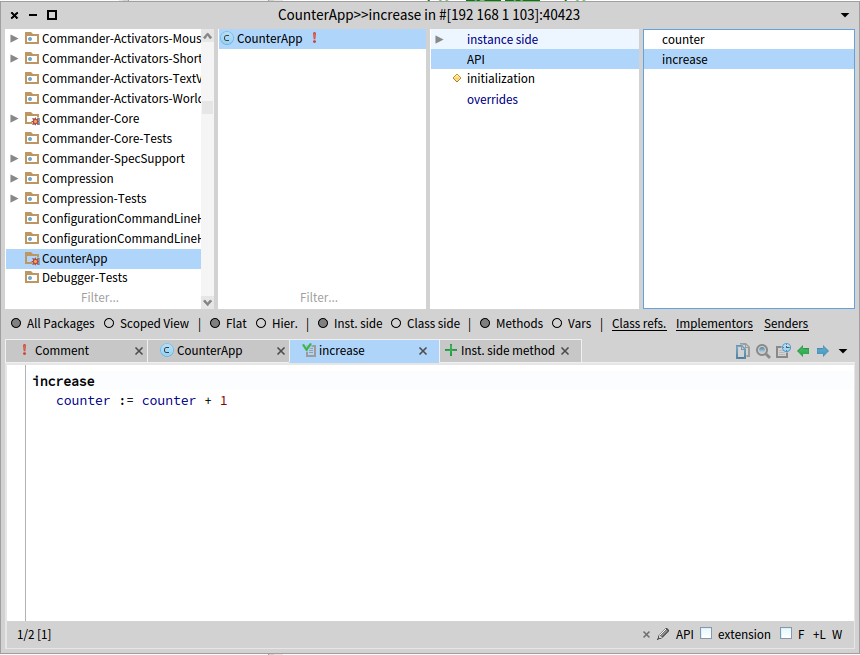
\includegraphics[scale=0.25]{../images/remote-browser}
	\end{center}	

\end{block}
}


\frame[containsverbatim]{\frametitle{Remote debugging}
\begin{block}{Live debugging of a remote application}
\begin{itemize}
				\item In your remote counter class, write the following method:			
\end{itemize}

\begin{lstlisting}
	decrease
	    counter := counter / 0
\end{lstlisting}	

\begin{itemize}
				\item Instantiate your counter in the remote playground
				\item Call the decrease method: there is an error because of the division by 0!
				\item Click "debug": a remote debugger opens
				\item Fix the method, then click "proceed"
				\item The remote code is modified and the execution continues!			
\end{itemize}


%	\begin{center}
%	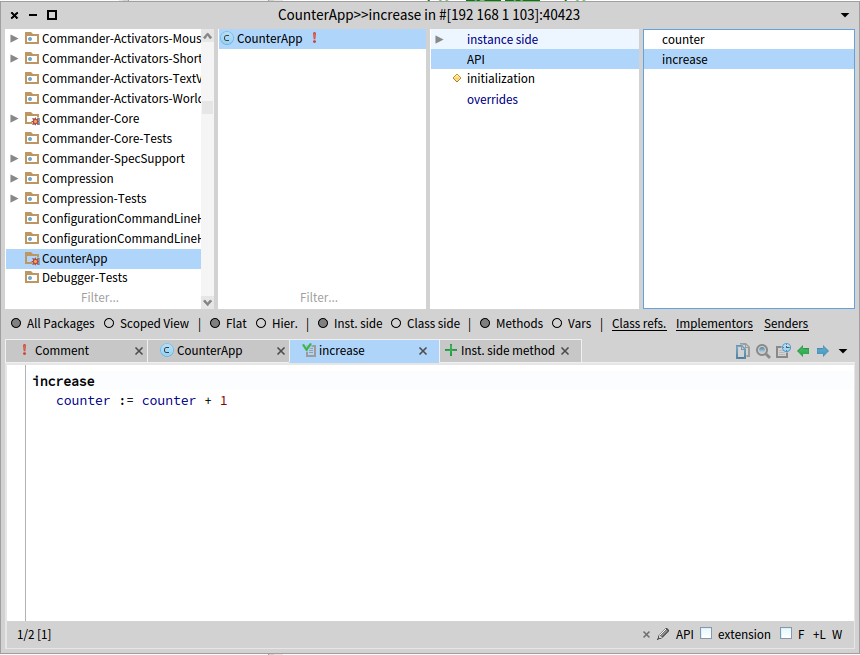
\includegraphics[scale=0.25]{../images/remote-browser}
%	\end{center}	

\end{block}

}

\frame{\frametitle{The remote process browser}
\begin{block}{Inspect and control processes running on your remote Pharo application}
\begin{itemize}
				\item Remotely open it using \texttt{remotePharo openProcessBrowser} 
				\item Process priorities are on the left
				\item Process names are displayed in the first column
				\item Process stacks are on the right
				\item The action bar in the middle allows you to control processes
\end{itemize}

	\begin{center}
		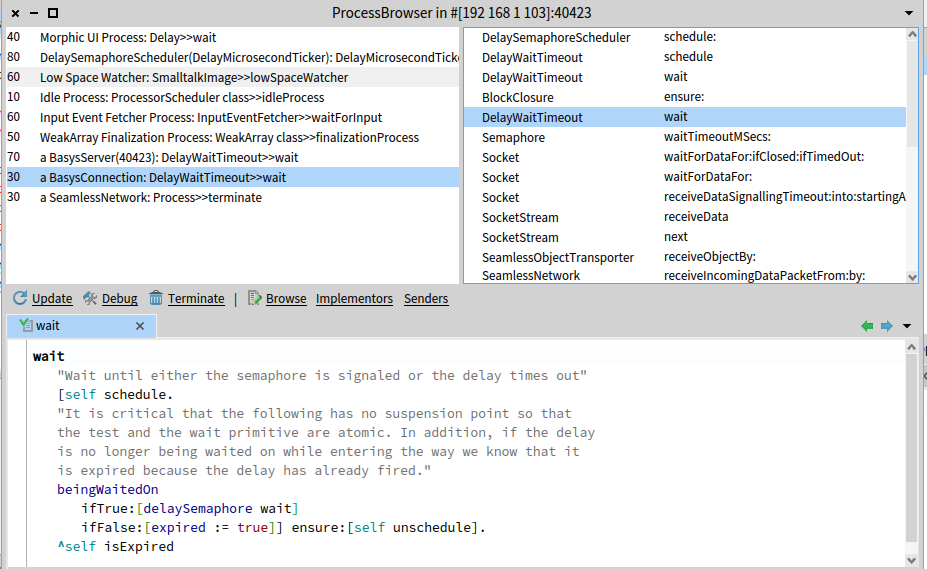
\includegraphics[scale=0.25]{../images/remote-process-browser}
	\end{center}	

\end{block}
}

\section{PharoThings exercises!}

\frame{\frametitle{Turning LEDs on and off}

\begin{block}{Follow and adapt code from tutorial chapter 2}
	\begin{columns}
		\begin{column}{0.48\textwidth}
			\begin{center}
				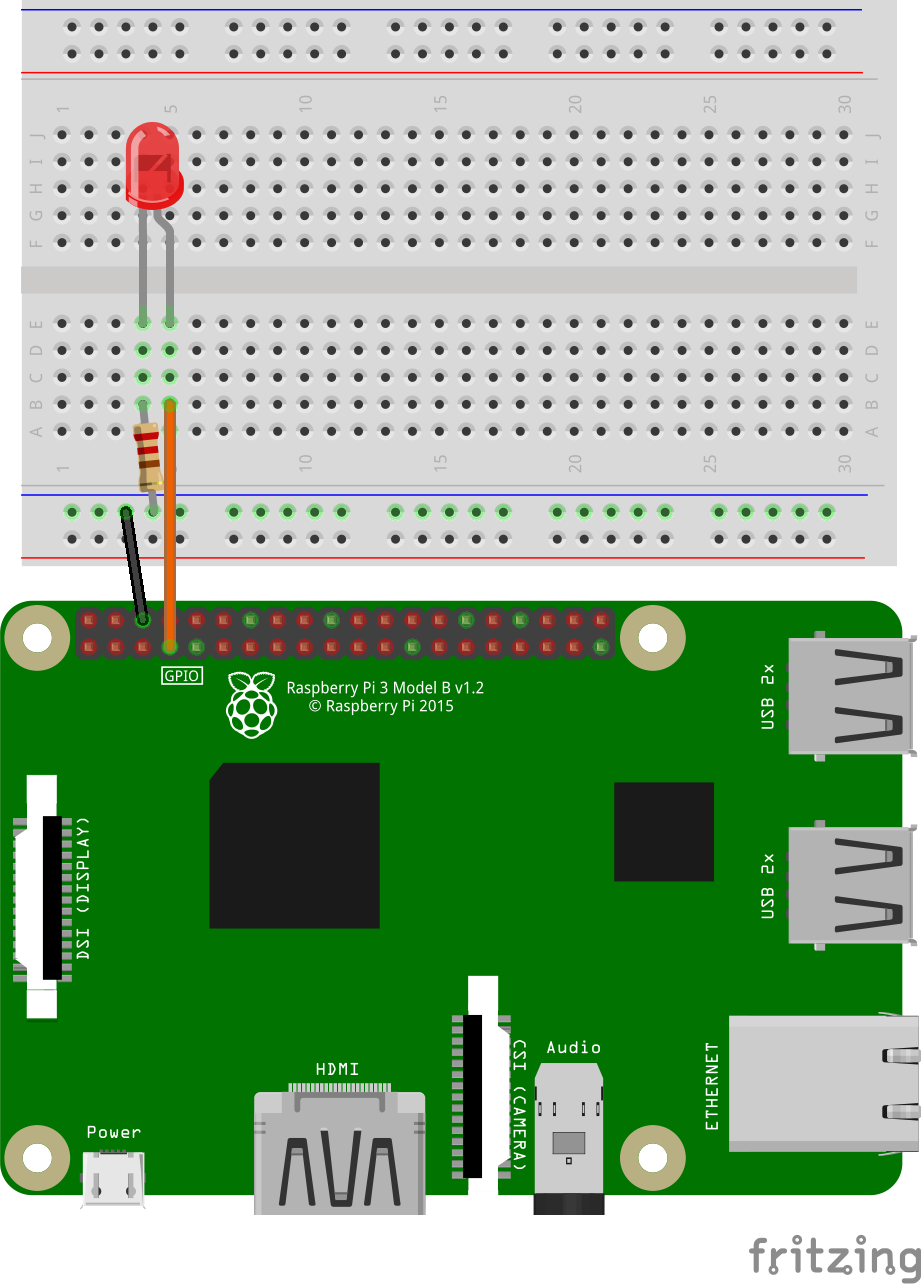
\includegraphics[width=1\textwidth]{../images/pharothings-raspberry-led-resistor-lesson-01}
			\end{center}
		\end{column}
	\begin{column}{0.48\textwidth}
	\begin{enumerate}
				\item Build the LED circuit
				\item Connect to the remote Pharo image
				\item Open a remote Raspberry-pi board inspector
				\item Set the LED pin to \texttt{HIGH}
				\item Play with \texttt{toggleDigitalValue} to toggle the LED pin state
\end{enumerate}
	\end{column}
	\end{columns}
\end{block}

}

\frame[containsverbatim]{\frametitle{Blinking a LED}

\begin{block}{Follow and adapt code from tutorial chapter 3}
	\begin{columns}
		\begin{column}{0.48\textwidth}
			\begin{enumerate}
				\item Reuse the previous lesson to set an output pin for the LED
				\item Write a loop that toogles the pin state
				\item Use a delay to wait between each iteration
				\item Create a process by forking the loop (and give it a name)
\end{enumerate}
		\end{column}
	\begin{column}{0.6\textwidth}
	\begin{lstlisting}
[10 timesRepeat: [
    led toggleDigitalValue.
    (Delay forSeconds: 1) wait
    ]
] forkNamed: 'BlinkerProcess'
\end{lstlisting}	
	\end{column}
	\end{columns}
\end{block}
}

\frame[containsverbatim]{\frametitle{Model your own LED blinker}

\begin{block}{The Device App model}
			\begin{itemize}
				\item The \texttt{PotAppDevice} class is a general model to implement devices that requires frequent updates\\
				\item Those devices have their own process\\
				\item Implemented by the \texttt{Blinker} class\\
				
				\begin{itemize}										
					\item Subclass the \texttt{PotAppDevice} class to implement your own device\\
					\item Implement the \texttt{loopBody} method: this is the behavior that will be executed after each delay\\		
					\item Control the process using \texttt{delay:}\\	
				\end{itemize}
		\end{itemize}
		
\end{block}
}

\frame[containsverbatim]{\frametitle{Model your own LED blinker}

\begin{block}{Implement the LED blinker as a Pharo-IOT app device!}
	
			\begin{itemize}
				\item We want a blinker object, that we can control!				
\end{itemize}

			\begin{enumerate}

				\item Create a \texttt{Blinker} class, subclass of \texttt{PotAppDevice} 
				\item Create an \texttt{initialize} method to set the initial state of the blinker
				\item You must be able to start and stop the blinking 
\end{enumerate}
	
\begin{lstlisting}
|blinker|
blinker := Blinker new.
blinker delay: 1 second.
blinker start. "start the blinker"
blinker stop. "stop the blinker"
\end{lstlisting}	

\end{block}
}

\frame[containsverbatim]{\frametitle{Make your LED breath using PWM}
%Breath speed
\begin{block}{Follow and adapt code from tutorial chapter 7}

			\begin{itemize}
				\item We want a to make a LED light up then fade away				
\end{itemize}

\begin{lstlisting}
|breathingLed|
breathingLed := BreathingLed new.
breathingLed breatheDelay: 10 milliSeconds.
breathingLed breatheFrom: 10 to: 25.
breathingLed startBreathing. 
\end{lstlisting}	

			\begin{enumerate}
				\item Create a \texttt{BreathingLed} class with the remote browser
				\item Configure the LED pin to PWM output:
				\begin{lstlisting}
led function: PotPWMFunction new.
led bePWMOutput.
\end{lstlisting}	
				\item The PWM value must be in the interval $[0, 1023]$:
								\begin{lstlisting}
led writePWMValue: 42.
\end{lstlisting}	
				\item To make the led breath, you must increment the PWM value by 1 from a \texttt{start} value in a loop until it reaches a \texttt{stop} value.
				When it does, decrease the value by 1 until it reaches the \texttt{start} value again, and so on.
\end{enumerate}

\begin{lstlisting}
|breathingLed|
breathingLed := BreathingLed new.
breathingLed delay: 10 milliSeconds.
breathingLed breathe. 
\end{lstlisting}	

\end{block}
}



\frame{\frametitle{Ultra-Sonic sensor: basic concepts}

%So is just to see how long time the ECHO pin will stay ON and calculate the distance because we already know the sound speed.
			\begin{itemize}
				\item The sensor sends an ultrasonic pulse, triggered by a 10 $\mu$s 5V signal on the \texttt{Trigger} pin
				\item Pulse waves reflect on objects in front and are reflected back to the sensor		
				\item The sensor detects these waves and sends a 5V signal on the \texttt{Echo} pin	
				\item The duration of the \texttt{echo} signal is proportional to the distance: 
				we can approximate the distance using the speed of sound ($\approx$340$m.s^{-1}$)			
			\end{itemize}

			\begin{center}
				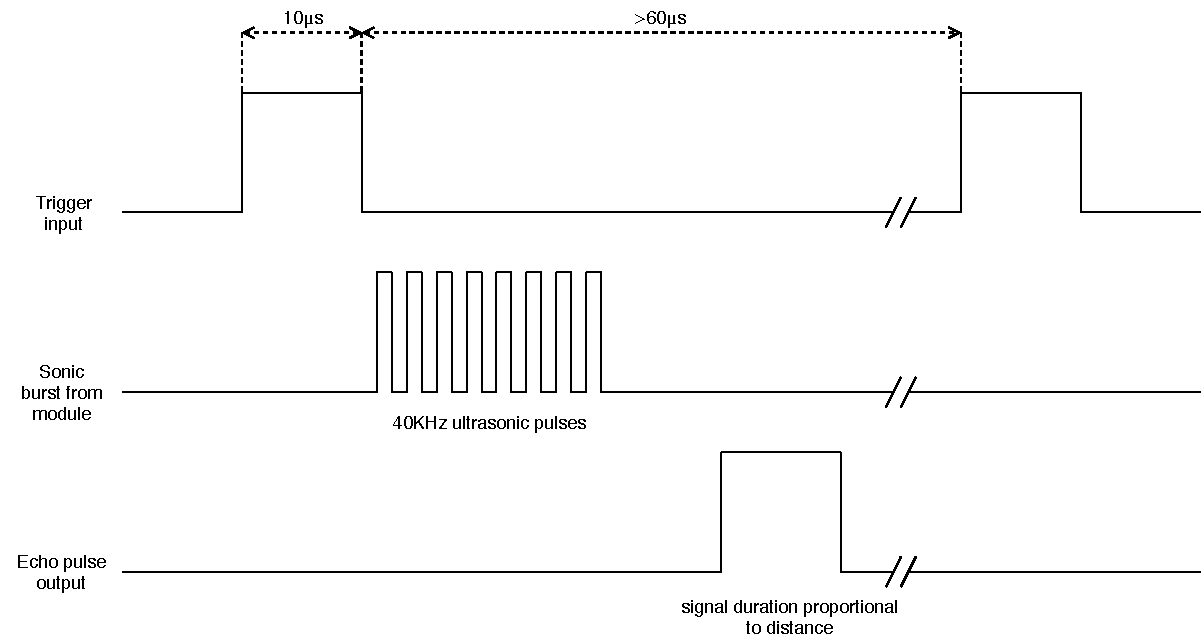
\includegraphics[scale=0.45]{../images/HSR04}
			\end{center}
}

\frame[containsverbatim]{\frametitle{Ultra-Sonic sensor: write your own driver!}

\begin{block}{Build the circuitry}
\begin{itemize}
				\item Follow instructions from chapter 10			
			\end{itemize}
\end{block}

\begin{block}{Write your own driver}
\begin{itemize}
				\item Create a class with two instance variables: an \texttt{echo} and a \texttt{trigger} pins
				\item Create an instance creation method to initialize the pins:
				\begin{lstlisting}
    sensor trigger: triggerPinId echo: echoPinId
				\end{lstlisting}
				\item Write the sensor behavior:
				\begin{enumerate}
				\item A method that sends a pulse
				\item A method that receives the pulse back signal and computes its duration
				\item A method that computes the distance from the pulse duration
				\item An interface method named \texttt{readDistance} that use all the previous method to return a distance (see next slide)		
			\end{enumerate}
				
					
				\item Test your sensor!		
			\end{itemize}
\end{block}
}

\frame[containsverbatim]{\frametitle{Write your own driver: the pulse back signal reception (1/2)}

\begin{block}{Concept of a \texttt{pulseIn}\footnote{\url{https://www.arduino.cc/reference/en/language/functions/advanced-io/pulsein/}}}
\begin{itemize}
				\item Reads a pulse (either \texttt{HIGH} or \texttt{LOW}) on a pin
				\item For example, if value is \texttt{HIGH}, waits for the pin to go from \texttt{LOW} to \texttt{HIGH}
				\item Starts a timer then waits for the pin to go \texttt{LOW} and stops timing
				\item Returns the length of the pulse in microseconds or gives up and returns 0 if no complete pulse was received within the timeout				
			\end{itemize}
\end{block}

\begin{alertblock}{In Pharo:}
\begin{itemize}
			\item We do not have the \texttt{pulseIn} mechanism in Pharo, therefore we have to simulate it!
\end{itemize}
\end{alertblock}

}

\frame[containsverbatim]{\frametitle{Write your own driver: the pulse back signal reception (2/2)}

\begin{block}{Simulated \texttt{pulseIn} in Pharo}

			
\textbf{Function:} pulseIn\\
\begin{algorithm}[H]  
\KwData{The Echo pin $echo$ set as digital input and with pull down resister enabled\footnote{\texttt{send the \texttt{enablePullDownResister} message to the pin object}}}
\KwResult{A duration}
  \Begin{
	\While{read($echo$) == 0}{$startTime\leftarrow$ currentTime}
	\While{read($echo$) == 1}{$endTime\leftarrow$ currentTime}
  	\Return $endTime - startTime$   
    }
\end{algorithm}
\end{block}


}

\frame[containsverbatim]{\frametitle{Write your own driver: the \texttt{readDistance} interface}

\begin{block}{Beware of timeouts!}
\begin{itemize}
				\item \textbf{Use a semaphore to avoid infinite waiting on timeouts!}			
			
\begin{lstlisting}		
readDistance 
    | travelTime semaphore |
    semaphore := Semaphore new.
    [ ...use the sensor to find travel time... ] fork.
    semaphore 
        wait: 100 milliSeconds
        onCompletion: [...return the travel time... ] 
        onTimeout: [ self rebootSensor. ^ -1 ]			
\end{lstlisting}

				\item \textbf{When the sensor times out, use the reboot trick:	}	
				\begin{lstlisting}		
rebootSensor
    echoPin beDigitalOutput; value: 1.
    1 milliSeconds wait.
    echoPin value: 0.
    echoPin  beDigitalInput; enablePullDownResister.
    triggerPin beDigitalOutput; value: 0			
\end{lstlisting}

\end{itemize}
	
\end{block}

}

\frame{\frametitle{Ultra-Sonic sensor: combine it with LED breathing!}

\begin{block}{Write an IOT application using an LED and an UltraSonic sensor}

			\begin{enumerate}
				\item When there is nothing closer than 1 meter, the LED is off
				\item When something is detected closer than 1 m, the light starts emitting light
				\item The closer the obstacle, the brighter must be the LED!
			\end{enumerate}
\end{block}
}

%\frame{\frametitle{A practical introduction with Pharo and PharoThings}
%\begin{block}{Schedule 2h00 - 6h00}
%\begin{itemize}
%		\item (2h00 - 2h30) I2C protocol/connecting Rasps
%		\item (2h30 - 3h00) Hands on BME280
%		\item (3h00 - 3h40) Hands on LCD
%		\item (3h40 - 4h00) Pause
%		\item (4h00 - 5h00) Mini weather station cloud
%		\item (5h00 - 6h00) Building a Webserver on Raspberry
%\end{itemize}

%	\begin{center}
%	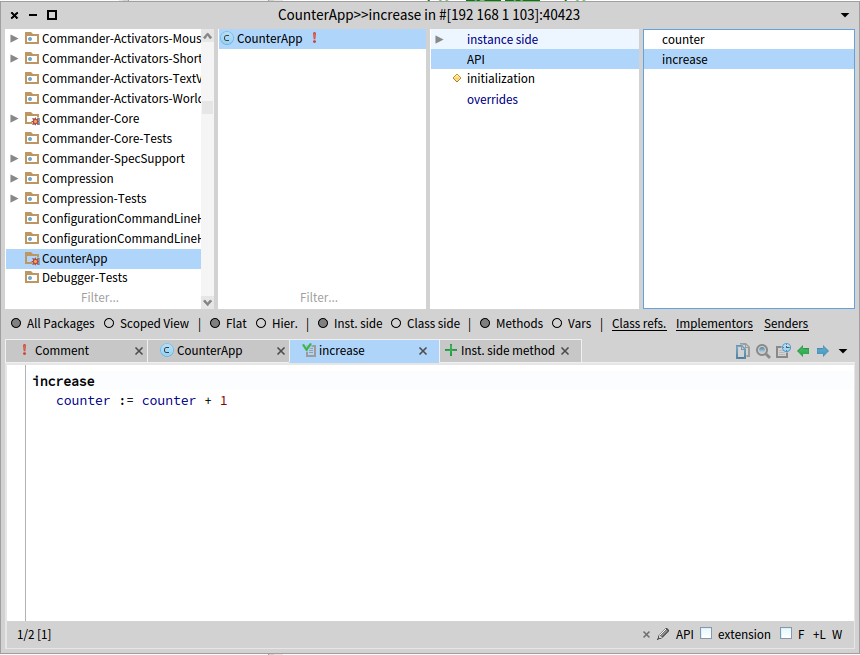
\includegraphics[scale=0.25]{../images/remote-browser}
%	\end{center}	

%\end{block}

%}

\frame{\frametitle{I2C Sensors}
\begin{block}{How I2C works?}
\begin{itemize}
		\item Use 2 wires SDA (serial data) and SCL (serial clock)
		\item Each device has set an ID or a unique address
		\item 112 devices using 7-bit addressing
		\item 1008 devices using 10-bit addressing		
\end{itemize}

%	\begin{center}
%	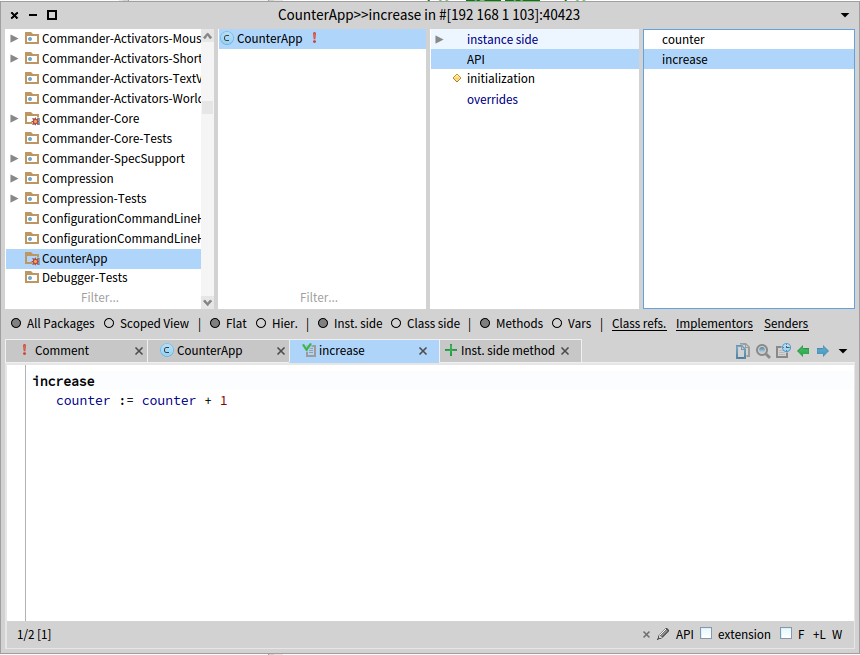
\includegraphics[scale=0.25]{../images/remote-browser}
%	\end{center}	

\end{block}

}

\frame{\frametitle{I2C Sensors}
\begin{block}{How I2C works?}
\begin{itemize}
		\item Use 2 wires SDA (serial data) and SCL (serial clock)
		\item Each device has set an ID or a unique address
		\item 112 devices using 7-bit addressing
		\item 1008 devices using 10-bit addressing		
\end{itemize}

	\begin{center}
	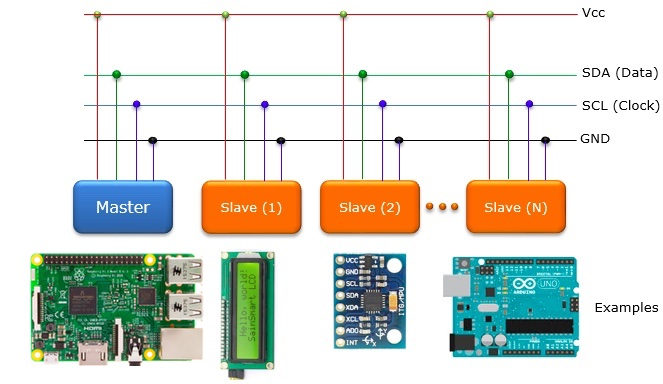
\includegraphics[scale=0.45]{../images/pharothings-i2c-bus.jpg}
	\end{center}	

\end{block}

}

\frame{\frametitle{I2C Sensors}
\begin{block}{I2C and GPIO based devices}
\begin{itemize}
		\item PotLCDHD44780 class
		\item Written to work with both models	
\end{itemize}

	\begin{center}
	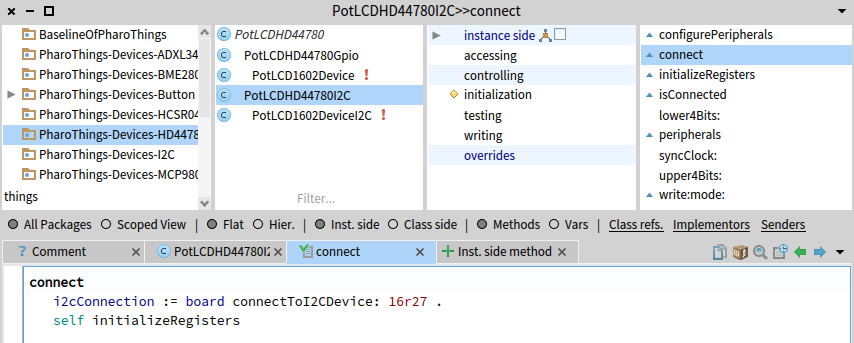
\includegraphics[scale=0.45]{../images/i2c-lcd-class.png}
	\end{center}	

\end{block}

}

\frame{\frametitle{I2C Sensors}
\begin{block}{BME280 sensor}
\begin{itemize}
		\item PotBME280Device class
\end{itemize}

	\begin{center}
	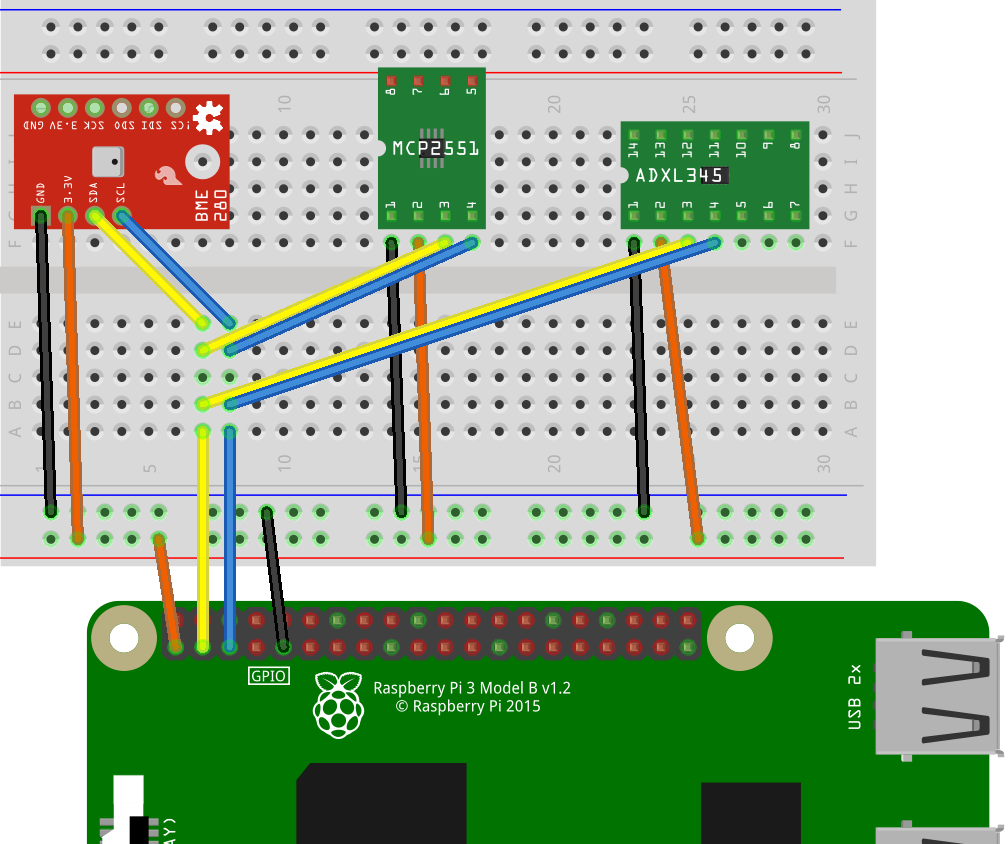
\includegraphics[scale=0.85]{../images/pharothings-sensors-board.png}
	\end{center}	

\end{block}

}

\frame{\frametitle{LCD screen}
\begin{block}{LCD 1602}
\begin{itemize}
		\item PotLCD1602Device class to GPIO device
		\item PotLCD1602DeviceI2C class to I2C device
\end{itemize}

	\begin{center}
	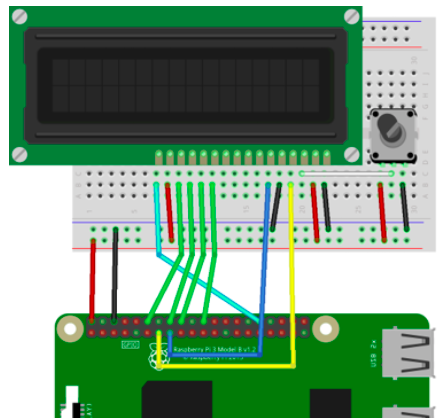
\includegraphics[scale=0.45]{../images/pharothings-lcd-board.png}
	\end{center}	

\end{block}
}

\frame{\frametitle{LCD screen}
\begin{block}{Write an IOT application using an LCD and an BME280 sensor}

			\begin{enumerate}
				\item Shows the data of sensor on the LCD each 1 second
			\end{enumerate}
\end{block}
}

\frame{\frametitle{Mini wheather station}
\begin{block}{Chapter 12 of Bookletr}

			\begin{enumerate}
				\item Create an account on Thingspeak
				\item Create the class to show the sensor data on LCD
				\item Create the class to send data to cloud
			\end{enumerate}
\end{block}
}

\frame{\frametitle{Web server}
\begin{block}{Chapter 13 of Bookletr}

			\begin{enumerate}
				\item Create the html page and start the webserver
				\item Create the methods to show the data on the web page
				\item Exercises, connect the sensor and LED to the web page
			\end{enumerate}
\end{block}
}


\end{document}

